\documentclass{article}
%----------------------------------------------------------------------------------------
%	PACKAGES AND DOCUMENT CONFIGURATIONS
%----------------------------------------------------------------------------------------


\usepackage{graphicx} % Required for the inclusion of images
\usepackage[square,sort,comma,numbers]{natbib}
\usepackage{amsmath} % Required for some math elements 

\usepackage{cmap}
\usepackage[T2A]{fontenc}
\usepackage[utf8x]{inputenc}
\usepackage[english, russian]{babel}

\usepackage{xcolor}
\usepackage{hyperref}
\usepackage{float}
\usepackage{listings}
\usepackage[left=30mm]{geometry} % настройки полей документа
\lstset{language=R, basicstyle=\small, extendedchars=\true, breaklines=true, breakatwhitespace=true} 

\hypersetup{pdfstartview=FitH, linkcolor=black, urlcolor=black, citecolor=black, colorlinks=true}

\setlength\parindent{0pt} % Removes all indentation from paragraphs

\renewcommand{\labelenumi}{\arabic{enumi}.}

\addto\captionsrussian{\def\refname{Литература}}

%----------------------------------------------------------------------------------------
%	DOCUMENT INFORMATION
%----------------------------------------------------------------------------------------
\begin{document}

\begin{titlepage}
	\begin{center}
		\textsc{Санкт-Петербургский политехнический университет\\Петра Великого\\[5mm]
			Физико-механический институт\\[2mm]
			Высшая школа прикладной математики и вычислительной физики}
		
		\vfill
		
		\textbf{Отчет\\по лабораторным работам №5-8\\по дисциплине\\ «Математическая статистика»
			\\[26mm]
		}
	\end{center}
	
	\begin{flushright}
		Выполнил студент: \\
		Иванова А.С. \\
		группа: 5030102/00101 \\
	\end{flushright}
	
	\begin{flushright}
		Проверил: \\
		к.ф.-м.н., доцент \\
		Баженов Александр Николаевич
	\end{flushright}
	
	\vspace*{\fill}
	\begin{center}
		Санкт-Петербург\\2023 г.
	\end{center}
\end{titlepage}
\newpage

\tableofcontents
\newpage

\listoffigures
\newpage

\listoftables
\newpage



\section{Постановка задачи}

Для 5 распределений: 

\begin{itemize}
	\item Нормальное распределение $N(x,0,1)$
	\item Распределение Коши $C(x,0,1)$
	\item Распределение Лапласа $L(x,0,\frac{1}{\sqrt{2}})$
	\item Распределение Пуассона $P(k,10)$
	\item Равномерное распределение $U(x,-\sqrt{3},\sqrt{3})$
\end{itemize}

\begin{enumerate}
	\item Сгенерировать выборки размером 10, 50 и 1000 элементов. Построить на одном рисунке гистограмму и график плотности распределения.
	
	\item Сгенерировать выборки размером 10, 100 и 1000 элементов. Для каждой выборки вычислить следующие статистические характеристики положения данных: $\overline{x}$, $med \, x$, $z_{R}$, $z_{Q}$,$z_{tr}$. Повторить такие вычисления 1000 раз для каждой выборки и найти среднее характеристик положения их квадратов: 
	\begin{equation}
		E(z)=\overline{z}
	\end{equation}
    Вычислить оценку дисперсии по формуле: 
    \begin{equation}
    	D(z)=\overline{z^{2}}-\overline{z}^{2}
    \end{equation}
    Представить полученные данные в виде таблиц.
    
    \item Сгенерировать выборки размером 20 и 100 элементов. \\
    Построить для них боксплот Тьюки. \\
    Для каждого распределения определить долю выбросов экспериментально (сгенерировав выборку, соответствующую распределению 1000 раз, и вычислив среднюю долю выбросов) и сравнить с результатами, полученными теоретически. 
    
    \item Сгенерировать выборки размером 20, 60 и 100 элементов. \\
    Построить на них эмпирические функции распределения и ядерные оценки плотности распределения на отрезке [-4;4] для непрерывных распределений и на отрезке [6;14] для распределения Пуассона.
    
\end{enumerate}
\newpage

\section{Теория}

\subsection{Рассматриваемые распределения}

Плотности вероятности рассматриваемых распределений: 

\begin{itemize}
	\item Нормальное распределение
	
	\begin{equation}
		N(x, 0, 0) = \tfrac{1}{ \sqrt{2\pi}}e^{-\tfrac{x^2}{2}}
	\end{equation}
	
	\item Распределение Коши
	
	\begin{equation}
		C(x, 0, 1) = \dfrac{1}{\pi}\dfrac{1}{1 + x^2}
	\end{equation}
	
	\item Распределение Лапласа
	
	\begin{equation}
		L(x, 0, \frac{1}{\sqrt{2}}) =\tfrac{1}{\sqrt{2}}e^{-\sqrt{2}|x|}
	\end{equation}
	
	\item Распределение Пуассона
	
	\begin{equation}
		P(k, 10) = \tfrac{10^k}{k!}e^{-10}
	\end{equation}
	
	\item Равномерное распределение
	
	\begin{equation}
		U(x, -\sqrt{3}, \sqrt{3}) =
		\begin{cases} 
			\;\; \dfrac{1}{2\sqrt{3}} \;\;\;\; \text{при} \;\;\;\; |x| \leq \sqrt{3}\\
			\,\,\,\:\;\; 0 \;\;\;\;\;\;\; \text{при} \;\;\;\; |x| > \sqrt{3}
		\end{cases}
	\end{equation}
	
\end{itemize}

\subsection{Гистограмма}

Множество значений, которое может принимать элемент выборки разбивается на несколько интервалов. Чаще всего эти интервалы берутся одинаковыми (но не обязательно). Данные интервалы откладываются на горизонтальной оси, затем над каждым рисуется прямоугольник. Если все интервалы одинаковые, то высота каждого прямоугольника пропорциональна числу элементов выборки, попадающих в соответствующий интервал. Если интервалы разные, то высота прямоугольника выбирается так, чтобы его площадь была пропорциональна числу элементов выборки, попавших в данный интервал.

\subsection{Вариационный ряд}

Вариационный ряд -- последовательность элементов выборки, расположенных в неубывающем порядке. Одинаковые элементы повторяются.

\subsection{Выборочные числовые характеристики}

\subsubsection{Характеристики положения}

\begin{itemize}
	\item Выборочное среднее
	
	\begin{equation} \label{eq:mean}
		\overline{x} = \tfrac{1}{n}\sum\limits_{i=1}^n x_i
	\end{equation}
	
	\item Выборочная медиана
	
	\begin{equation} \label{eq:med}
		med \: x = 
		\begin{cases} 
			\;\;\;\;\;\;\; x_{(l+1)} \:\;\;\;\;\;\;\;\;\; \text{при} \;\;\;\; n = 2l + 1\\
			\;\; \dfrac{x_{(l)} + x_{(l+1)}}{2} \;\;\;\; \text{при} \;\;\;\; n = 2l
		\end{cases}
	\end{equation}
	
	\item Полусумма экстремальных выборочных элементов
	
	\begin{equation} \label{eq:zR}
		z_R = \dfrac{x_{(1)} + x_{(n)}}{2}
	\end{equation}
	
	\item Полусумма квартилей
	
	Выборочная квартиль $z_p$ порядка $p$ определяется формулой
	
	\begin{equation}
		z_p =
		\begin{cases}
			\;\; x_{([np]+1)} \;\;\;\; \text{при} \;\; np \;\; \text{дробном},\\
			\;\;\;\;\; x_{(np)} \,\:\;\;\;\;\; \text{при} \;\; np \;\; \text{целом}.
		\end{cases}
	\end{equation}
	
	Полусумма квартилей
	
	\begin{equation} \label{eq:zQ}
		z_Q = \dfrac{z_{1/4} + z_{3/4}}{2}
	\end{equation}
	
	\item Усечённое среднее
	
	\begin{equation} \label{eq:zTr}
		z_{tr} = \tfrac{1}{n-2r}\sum\limits_{i=r+1}^{n-r} x_{(i)}, \;\;\;\; r \approx \dfrac{n}{4}
	\end{equation}
	
\end{itemize}

\subsubsection{Характеристики рассеяния}

Выборочная дисперсия

\begin{equation}
	D = \tfrac{1}{n}\sum\limits_{i=1}^{n} (x_i - \overline{x})^2
\end{equation}

\subsection{Боксплот Тьюки}

\subsubsection{Построение}

Границы ящика -- первый и третий квартили, линия в середине ящика -- медиана. Концы усов -- края статистически значимой выборки (без выбросов). Длина "усов": 

\begin{equation} \label{eq:boundBoxplot}
	X_1 = Q_1 - \dfrac{3}{2}(Q_3 - Q_1), \;\; X_2 = Q_3 + \dfrac{3}{2}(Q_3 - Q_1),
\end{equation}

где $X_1$ --- нижняя граница уса, $X_2$ --- верхняя граница уса, $Q_1$ --- первый квартиль, $Q_3$ --- третий квартиль.

Данные, выходящие за границы усов (выбросы), отображаются на графике в виде маленьких кружков.

\subsection{Теоретическая вероятность выбросов}

Можно вычислить теоретические первый и третий квартили распределений ($Q_1^\text{т}$ и $Q_3^\text{т}$ соответственно). По формуле \eqref{eq:boundBoxplot} можно вычислить теоретические нижнюю и верхнюю границы уса ($X_1^\text{т}$ и $X_2^\text{т}$ соответственно). Выбросами считаются величины $x$, такие что:

\begin{equation}
	\left[ 
	\begin{gathered} 
		x < X_1^\text{т}\\ 
		x > X_2^\text{т}\\ 
	\end{gathered} 
	\right.
\end{equation}

Теоретическая вероятность выбросов для непрерывных распределений

\begin{equation} \label{eq:probTheorCont}
	P_\text{в}^\text{т} = P(x < X_1^\text{т}) + P(x > X_2^\text{т}) = F(X_1^\text{т}) + \Big(1 - F(X_2^\text{т})\Big),
\end{equation}

где $F(X) = P(x \le X)$ - функция распределения.\\

Теоретическая вероятность выбросов для дискретных распределений

\begin{equation} \label{eq:probTheorDisc}
	P_\text{в}^\text{т} = P(x < X_1^\text{т}) + P(x > X_2^\text{т}) = \Big(F(X_1^\text{т}) - P(x = X_1^\text{т})\Big) + \Big(1 - F(X_2^\text{т})\Big),
\end{equation}

где $F(X) = P(x \le X)$ - функция распределения.



\newpage

\section{Реализация}

Лабораторная работа была выполнена с помощью встроенных средств языка программирования Python (библиотеки: NumPy, SciPy, Matplotlib, Pandas) в среде разработки Visual Studio Code. Исходный код работы приведен в приложении.\\

Ссылка на репозиторий с исходным кодом: \url{https://github.com/anivse/MathematicalStatistics}


\newpage

\section{Результаты}

\subsection{Гистограмма и график плотности распределения}


\begin{figure}[H]
	\begin{tabular}{ccc}
		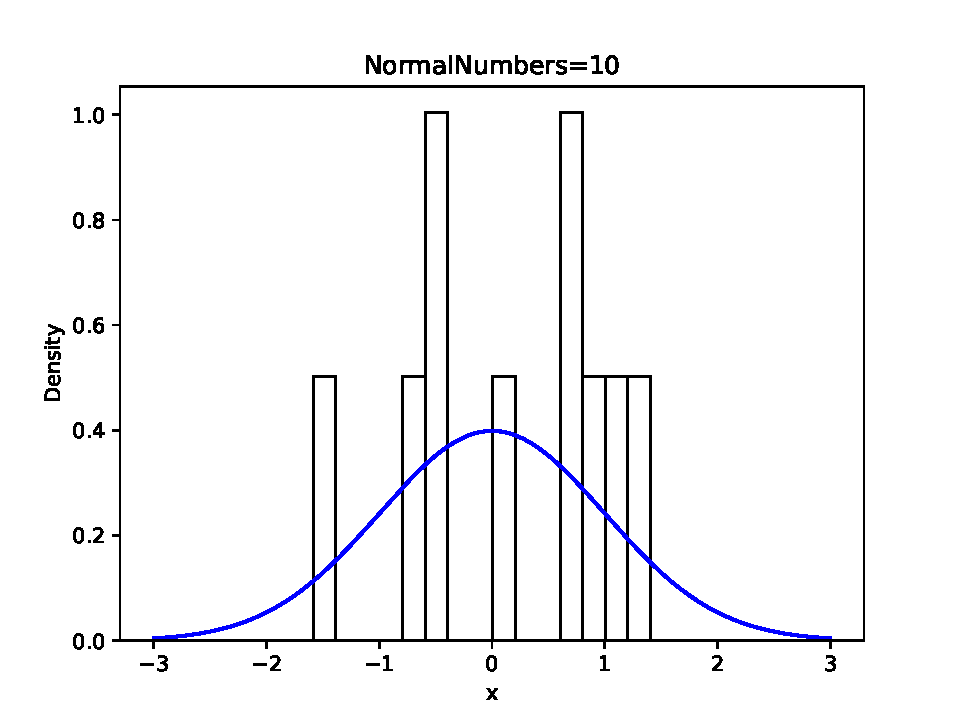
\includegraphics[scale=0.33]{normal_hist_10.pdf}
		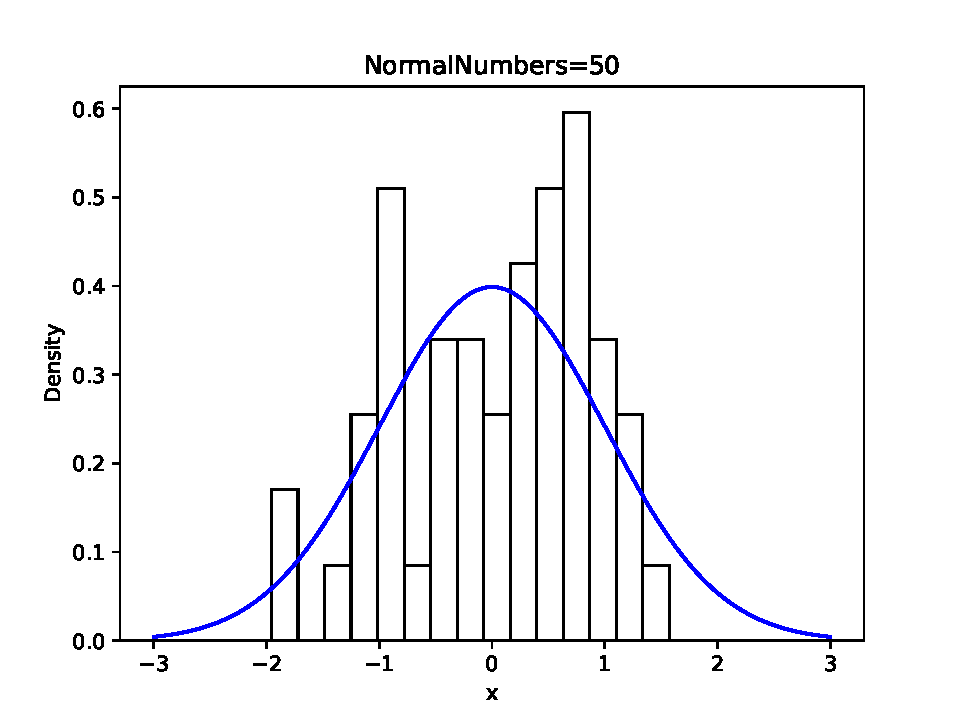
\includegraphics[scale=0.33]{normal_hist_50.pdf}
		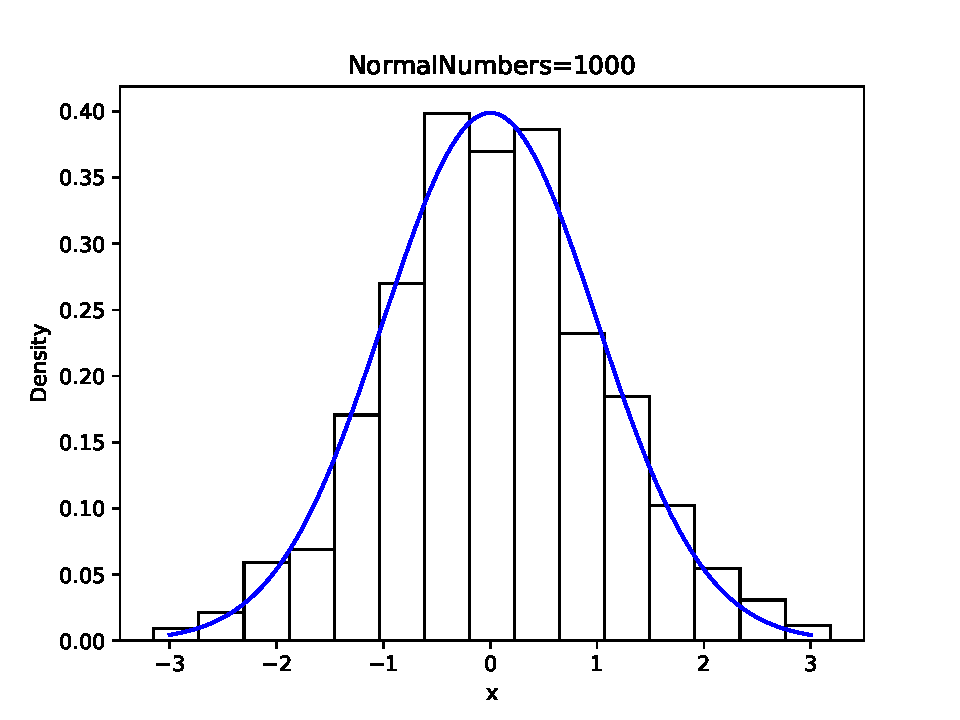
\includegraphics[scale=0.33]{normal_hist_1000.pdf}
	\end{tabular}
	\caption{Нормальное распределение}
\end{figure}

\begin{figure}[H]
	\begin{tabular}{ccc}
		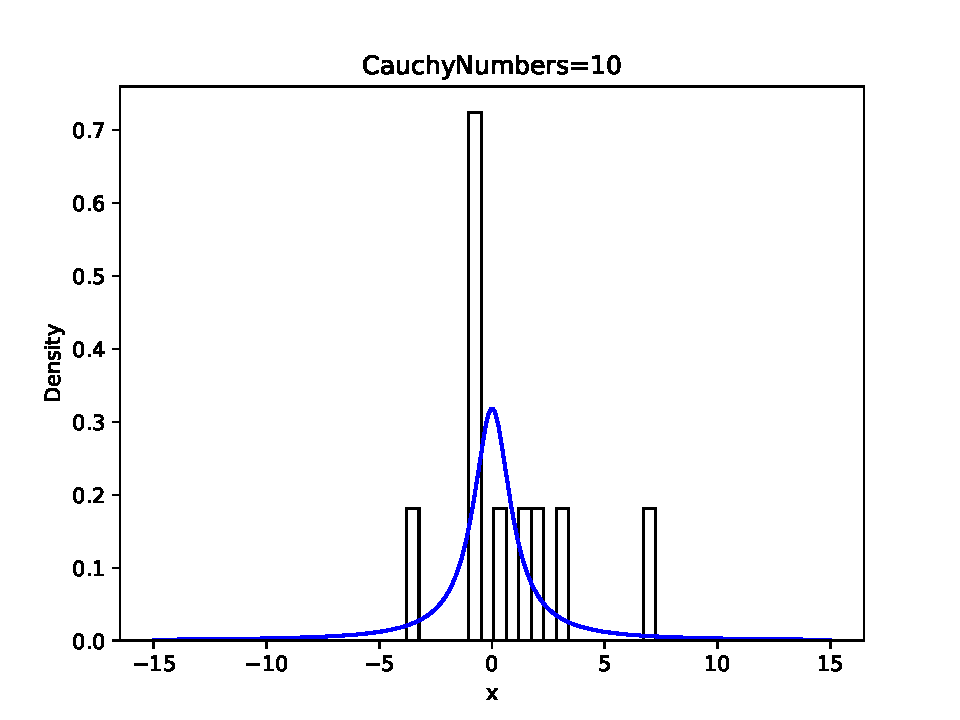
\includegraphics[scale=0.33]{cauchy_hist_10.pdf}
		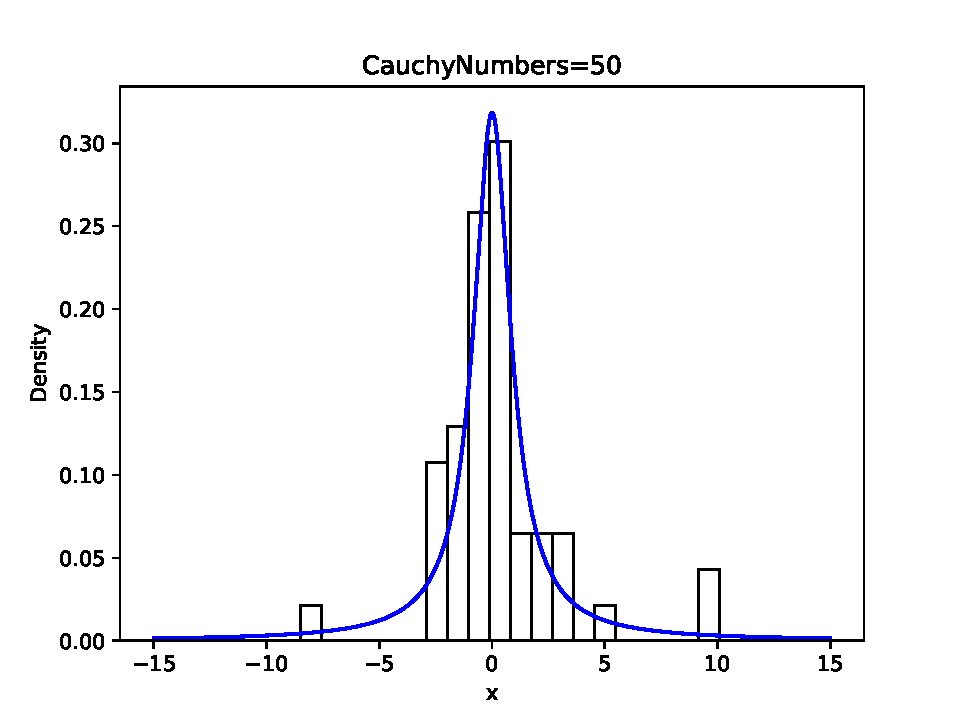
\includegraphics[scale=0.33]{cauchy_hist_50.pdf}
		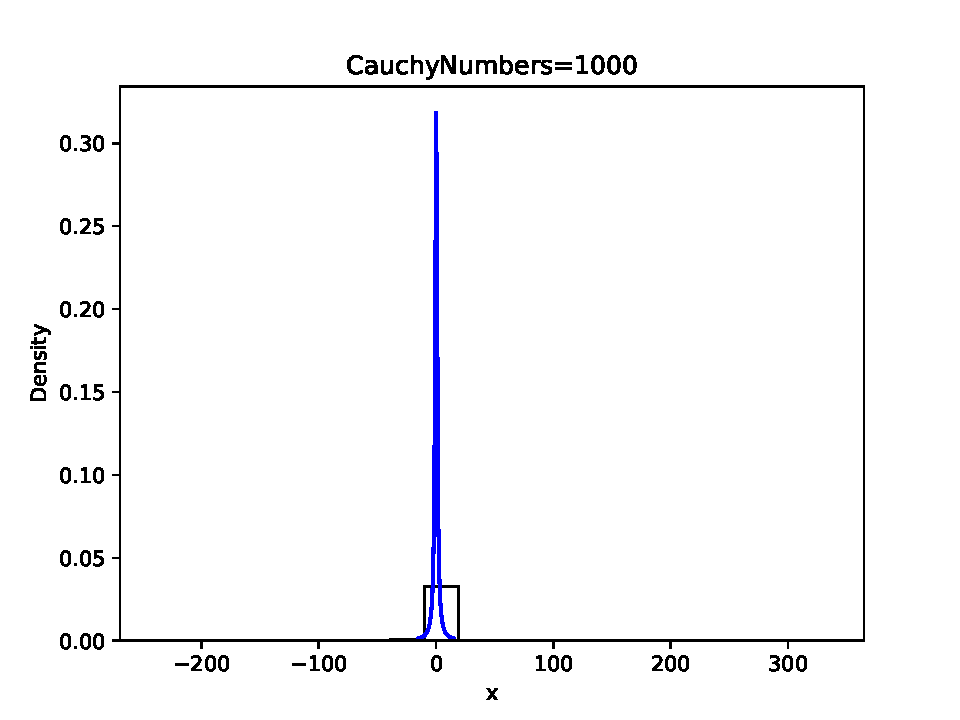
\includegraphics[scale=0.33]{cauchy_hist_1000.pdf}
	\end{tabular}
	\caption{Распределение Коши}
\end{figure}

\begin{figure}[H]
	\begin{tabular}{ccc}
		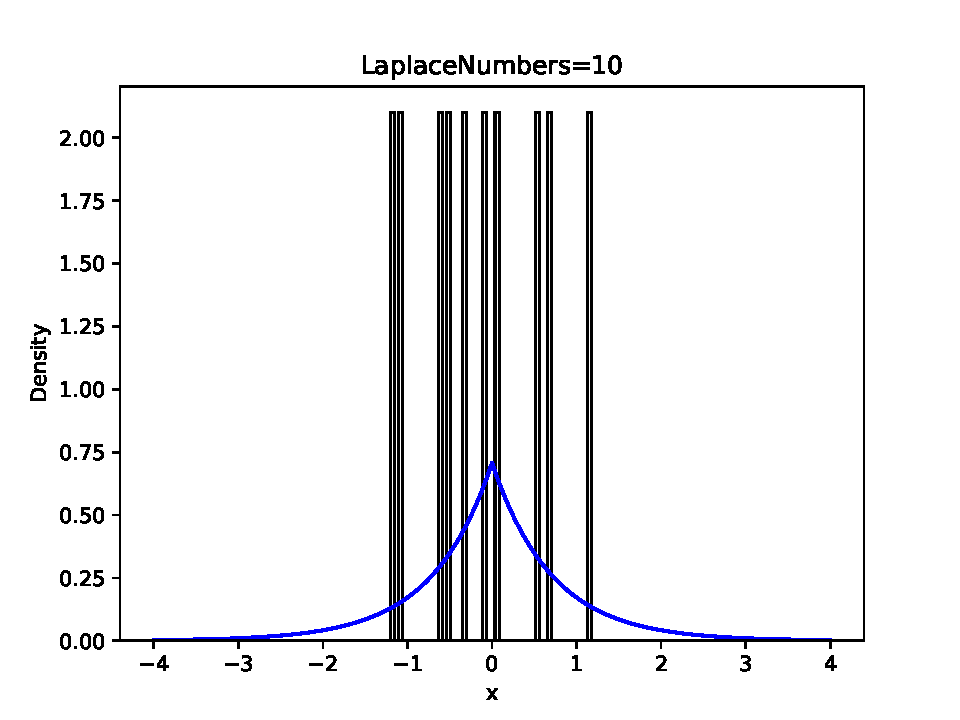
\includegraphics[scale=0.33]{laplace_hist_10.pdf}
		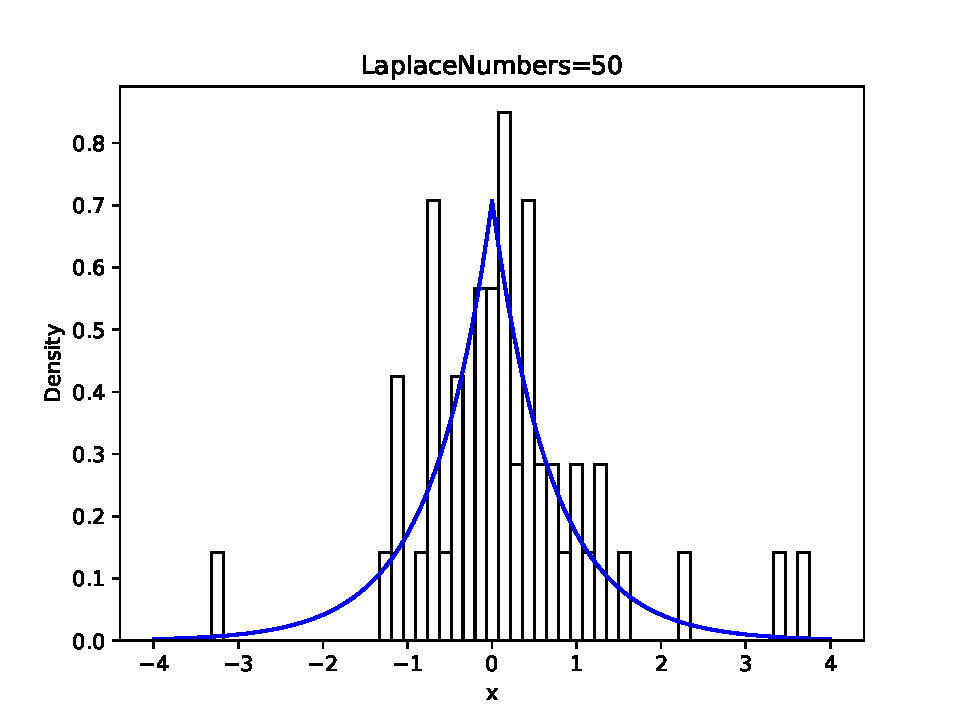
\includegraphics[scale=0.33]{laplace_hist_50.pdf}
		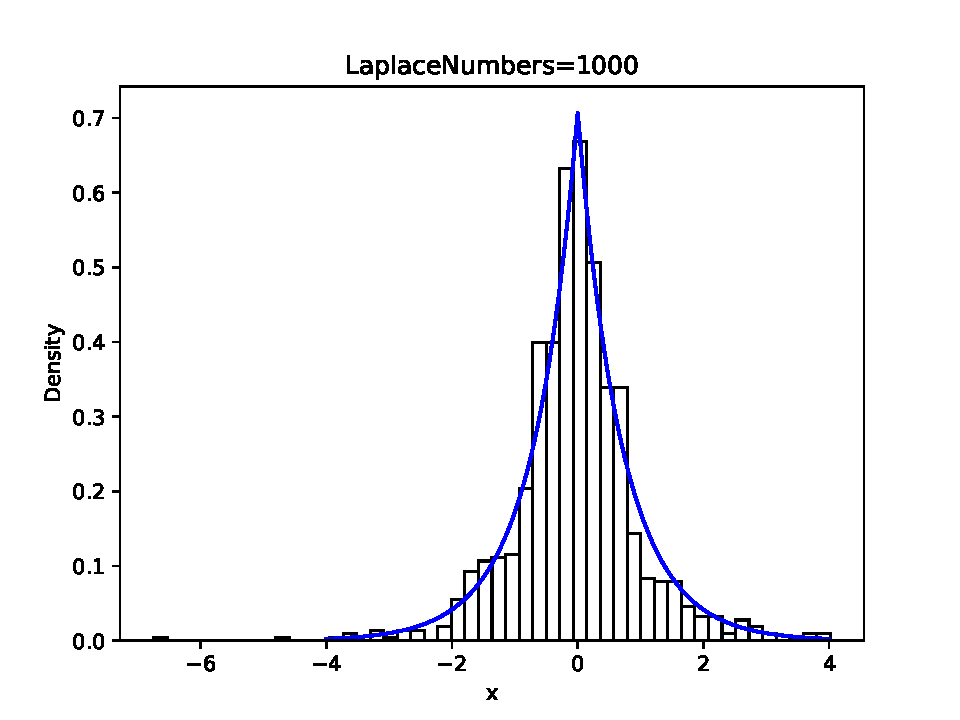
\includegraphics[scale=0.33]{laplace_hist_1000.pdf}
	\end{tabular}
	\caption{Распределение Лапласа}
\end{figure}

\begin{figure}[H]
	\begin{tabular}{ccc}
		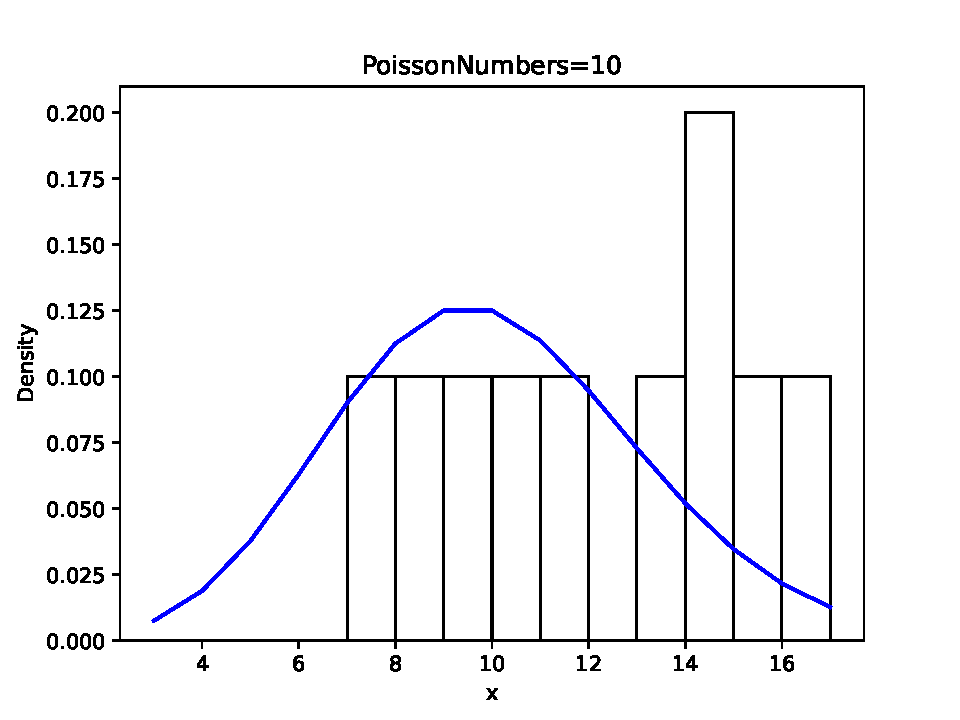
\includegraphics[scale=0.33]{poisson_hist_10.pdf}
		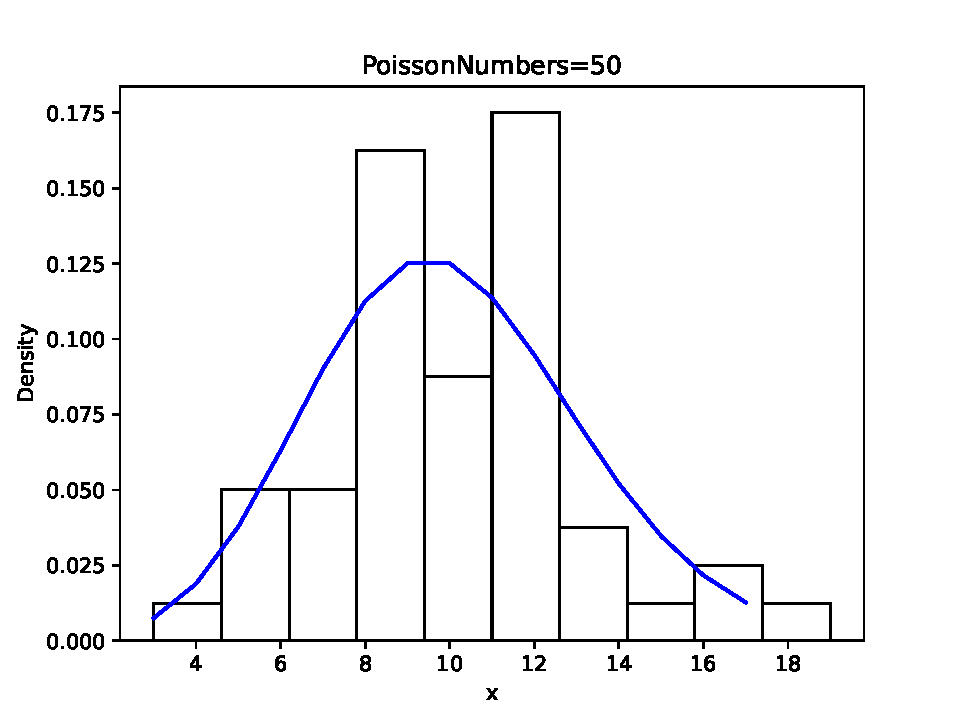
\includegraphics[scale=0.33]{poisson_hist_50.pdf}
		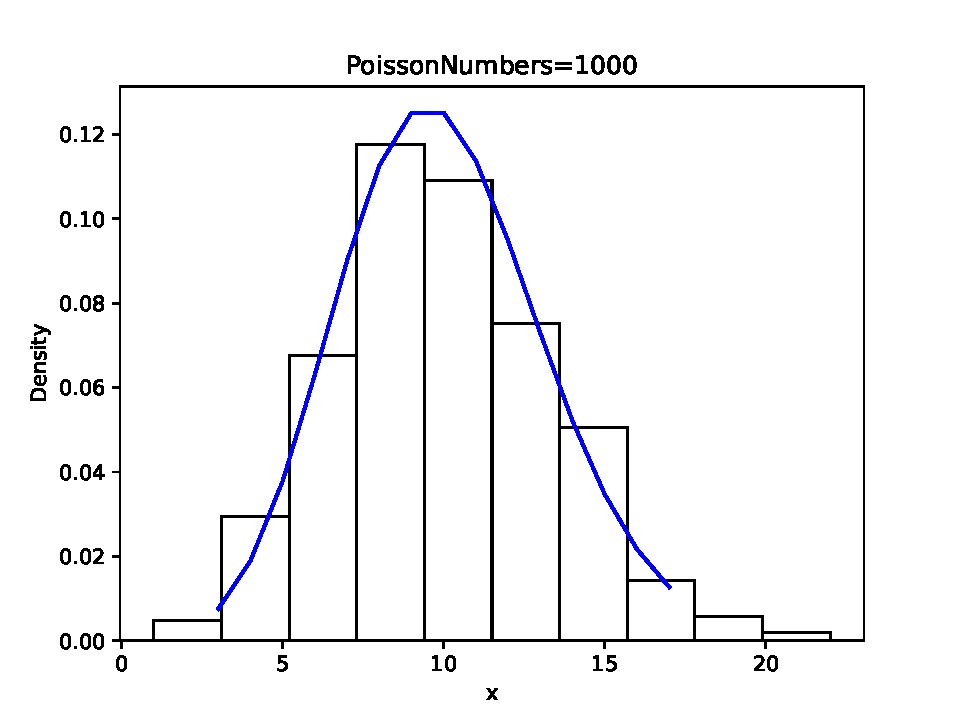
\includegraphics[scale=0.33]{poisson_hist_1000.pdf}
	\end{tabular}
	\caption{Распределение Пуассона}
\end{figure}


\begin{figure}[H]
	\begin{tabular}{ccc}
		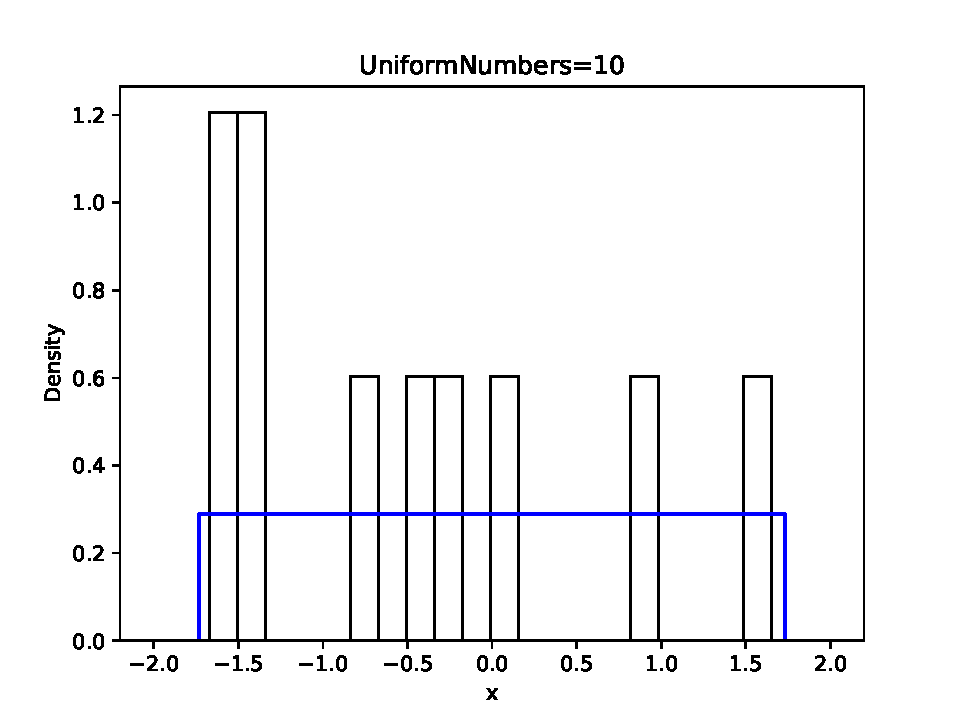
\includegraphics[scale=0.33]{uniform_hist_10.pdf}
		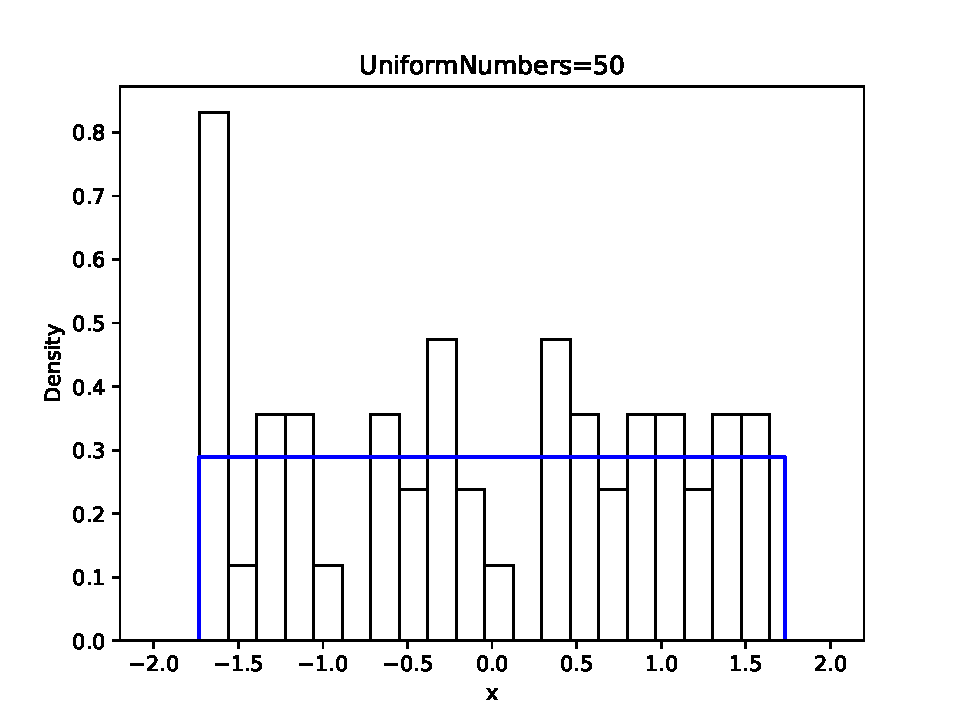
\includegraphics[scale=0.33]{uniform_hist_50.pdf}
		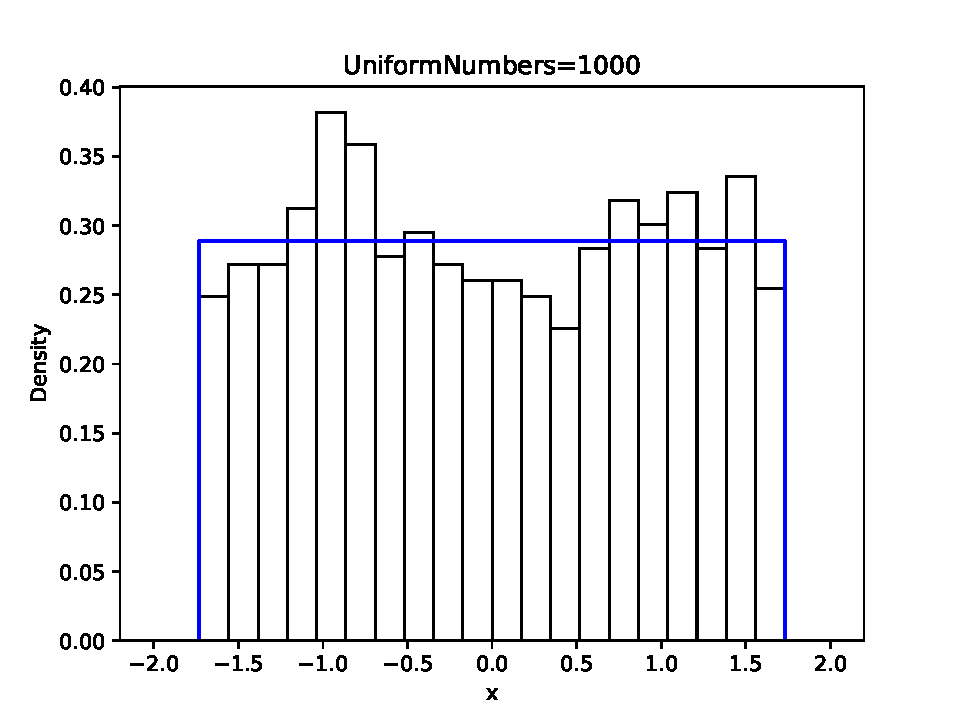
\includegraphics[scale=0.33]{uniform_hist_1000.pdf}
	\end{tabular}
	\caption{Равномерное распределение}
\end{figure}


\subsection{Характеристики положения и рассеяния}


 

\begin{table}[H]
	\begin{center}
		\begin{tabular}{|c||c|c|c|c|c|}
			\hline
			Normal n=10 & $\overline{x} $ & $med\:x$ & $z_{R}$ & $z_{Q}$ & $z_{tr}$ \\
			\hline\hline
			$E(z)$ & 0.00369 & 0.00140 & 0.00253 & 0.00218 & 0.00621 \\
			\hline
			$D(z)$ & 0.09933 & 0.13162 & 0.18904 & 0.12373 & 0.11933 \\
			\hline\hline
			Normal n=100 & $\overline{x} $ & $med\:x$ & $z_{R}$ & $z_{Q}$ & $z_{tr}$ \\
			\hline\hline
			$E(z)$ & -0.00061 & 0.00180 & 0.00675 & -0.01403 & -0.00010 \\
			\hline
			$D(z)$ & 0.00950 & 0.01575&  0.08953& 0.01197 & 0.01167  \\
			\hline\hline
			Normal n=1000 & $\overline{x} $ & $med\:x$ & $z_{R}$ & $z_{Q}$ & $z_{tr}$ \\
			\hline\hline
			$E(z)$ & -2.21952 & -0.00053 & -0.01664 & -0.00134 &   -0.00042 \\
			\hline
			$D(z)$ & 0.00101  & 0.00164 & 0.06311  &0.00124  & 0.00122 \\
			\hline
		\end{tabular}
	\end{center}
	\caption{Характеристики положения и рассеяния нормального распределения}
\end{table} 

\begin{table}[H]
	\begin{center}
		\begin{tabular}{|c||c|c|c|c|c|}
			\hline
			Cauchy n=10 & $\overline{x} $ & $med\:x$ & $z_{R}$ & $z_{Q}$ & $z_{tr}$ \\
			\hline\hline
			$E(z)$ & 0.60631 & -0.01793& 3.07935 & 0.00118 & -0.02171 \\
			\hline
			$D(z)$ & 3825.12746 & 0.36398 & 95430.01133 & 1.47888 & 0.38230 \\
			\hline\hline
			Cauchy n=100 & $\overline{x} $ & $med\:x$ & $z_{R}$ & $z_{Q}$ & $z_{tr}$ \\
			\hline\hline
			$E(z)$ & 0.68621 & -0.00218 & 33.379 & -0.02695 & 0.00145 \\
			\hline
			$D(z)$ &415.87354  &0.02449 & 1025245.02557 & 0.05200 &  0.02604\\
			\hline\hline
			Cauchy n=1000 & $\overline{x} $ & $med\:x$ & $z_{R}$ & $z_{Q}$ & $z_{tr}$ \\
			\hline\hline
			$E(z)$ & 0.02740 &-0.00038 & -5.55196 & -0.00173 & 7.45726 \\
			\hline
			$D(z)$ & 118.83309 &0.00243 & 28306188.93642 & 0.00501 &0.00252  \\
			\hline
		\end{tabular}
	\end{center}
	\caption{Характеристики положения и рассеяния распределения Коши}
\end{table}

\begin{table}[H]
	\begin{center}
		\begin{tabular}{|c||c|c|c|c|c|}
			\hline
			Laplace n=10 & $\overline{x} $ & $med\:x$ & $z_{R}$ & $z_{Q}$ & $z_{tr}$ \\
			\hline\hline
			$E(z)$ & 0.01279 &0.00579 & 0.02646 & 0.01273 & 0.00412 \\
			\hline
			$D(z)$ & 0.09453 &  0.07397 &  0.40262 &0.09303  &  0.06910 \\
			\hline\hline
			Laplace n=100 & $\overline{x} $ & $med\:x$ & $z_{R}$ & $z_{Q}$ & $z_{tr}$ \\
			\hline\hline
			$E(z)$ &0.00358  & 0.00157&0.00132  & -0.01101 & 0.00213 \\
			\hline
			$D(z)$ & 0.00990 &0.00523 & 0.42664 & 0.00966 & 0.00588 \\
			\hline\hline
			Laplace n=1000 & $\overline{x} $ & $med\:x$ & $z_{R}$ & $z_{Q}$ & $z_{tr}$ \\
			\hline\hline
			$E(z)$ & -0.00036 & 1.53039 & -0.01446 & -0.00114 & 0.00018 \\
			\hline
			$D(z)$ & 0.00102 &0.00050 & 0.41539 & 0.00096 & 0.00058  \\
			\hline
		\end{tabular}
	\end{center}
	\caption{Характеристики положения и рассеяния распределения Лапласа}
\end{table} 

\begin{table}[H]
	\begin{center}
		\begin{tabular}{|c||c|c|c|c|c|}
			\hline
			Poisson n=10 & $\overline{x} $ & $med\:x$ & $z_{R}$ & $z_{Q}$ & $z_{tr}$ \\
			\hline\hline
			$E(z)$ & 9.97609 &9.8235 & 10.2955 & 9.9105 &  9.8415  \\
			\hline
			$D(z)$ &0.97231  &1.37659 &1.79642 & 1.22023 & 1.21450 \\
			\hline\hline
			Poisson n=100 & $\overline{x} $ & $med\:x$ & $z_{R}$ & $z_{Q}$ & $z_{tr}$ \\
			\hline\hline
			$E(z)$ & 9.98505 & 9.836 & 10.9405  & 9.8475 & 9.84008 \\
			\hline
			$D(z)$ & 0.10400 & 0.22110 & 0.99120  & 0.16499 & 0.12406 \\
			\hline\hline
			Poisson n=1000 & $\overline{x} $ & $med\:x$ & $z_{R}$ & $z_{Q}$ & $z_{tr}$ \\
			\hline\hline
			$E(z)$ & 9.99791 & 9.9965 & 11.639 & 9.992  & 9.85761 \\
			\hline
			$D(z)$ &  0.00964 & 0.00323 & 0.61767 & 0.00443 & 0.01066 \\
			\hline
		\end{tabular}
	\end{center}
	\caption{Характеристики положения и рассеяния распределения Пуассона}
\end{table} 

\begin{table}[H]
	\begin{center}
		\begin{tabular}{|c||c|c|c|c|c|}
			\hline
			Uniform n=10 & $\overline{x} $ & $med\:x$ & $z_{R}$ & $z_{Q}$ & $z_{tr}$ \\
			\hline\hline
			$E(z)$ & 0.00336 &0.00843 & 0.00505 & -0.00111 & 0.00502 \\
			\hline
			$D(z)$ & 0.10159  & 0.22721 & 0.04560 & 0.14254 & 0.19700 \\
			\hline\hline
			Uniform n=100 & $\overline{x} $ & $med\:x$ & $z_{R}$ & $z_{Q}$ & $z_{tr}$ \\
			\hline\hline
			$E(z)$ & 0.00098 & 0.00587 & 0.00060 & -0.01393 &  0.00199\\
			\hline
			$D(z)$ & 0.01036 & 0.03018 & 0.00057 & 0.01545 & 0.02068  \\
			\hline\hline
			Uniform n=1000 & $\overline{x} $ & $med\:x$ & $z_{R}$ & $z_{Q}$ & $z_{tr}$ \\
			\hline\hline
			$E(z)$ & -0.00111 &-0.00171 & -0.00003 & -0.00240 & -0.00139  \\
			\hline
			$D(z)$ & 0.00100 & 0.00288 & 5.99778 & 0.00154 & 0.00198 \\
			\hline
		\end{tabular}
	\end{center}
	\caption{Характеристики положения и рассеяния равномерного распределения}
\end{table} 

\subsection{Боксплот Тьюки}

\begin{figure}[H]
	\centering
	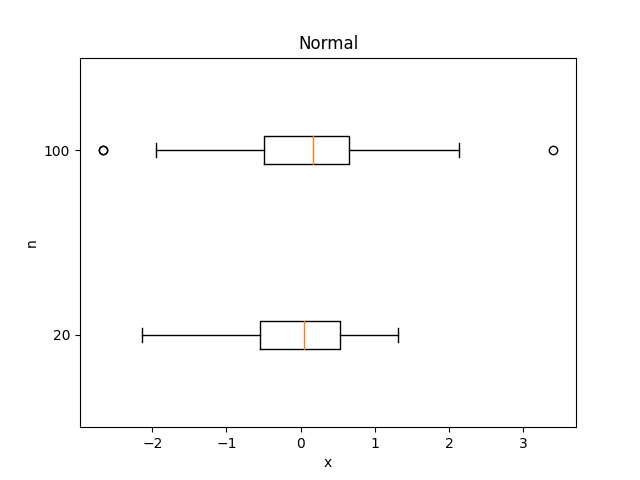
\includegraphics[scale=0.65]{normal_boxplot.png}
	\caption{Боксплот нормального распределения}
\end{figure}

\begin{figure}[H]
	\centering
	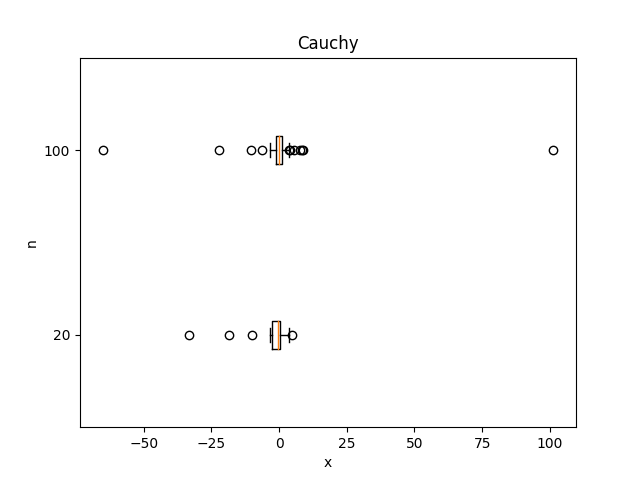
\includegraphics[scale=0.65]{cauchy_boxplot.png}
	\caption{Боксплот распределения Коши}
\end{figure}

\begin{figure}[H]
	\centering
	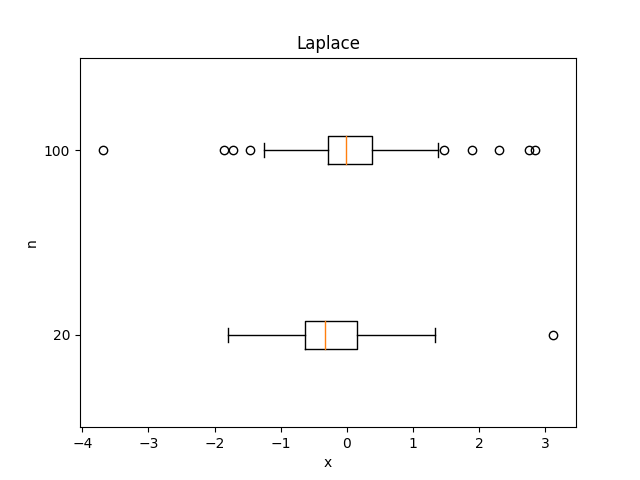
\includegraphics[scale=0.65]{laplace_boxplot.png}
	\caption{Боксплот распределения Лапласа}
\end{figure}

\begin{figure}[H]
	\centering
	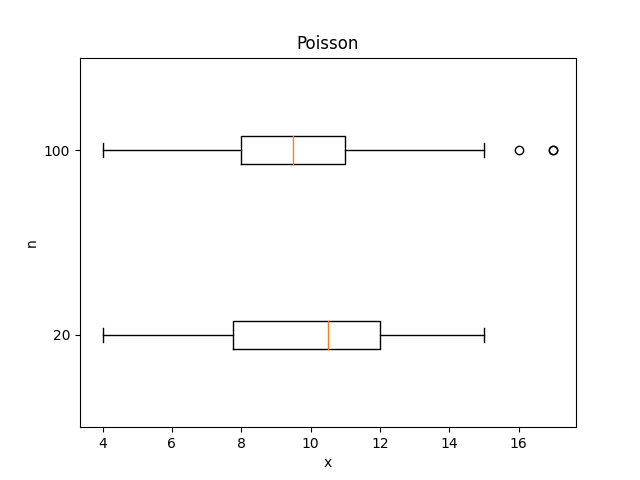
\includegraphics[scale=0.65]{poisson_boxplot.png}
	\caption{Боксплот распределения Пуассона}
\end{figure}

\begin{figure}[H]
	\centering
	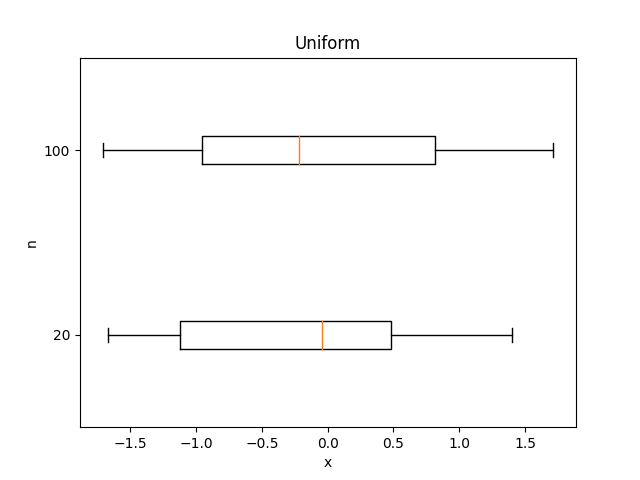
\includegraphics[scale=0.65]{uniform_boxplot.png}
	\caption{Боксплот равномерного распределения}
\end{figure}

\subsection{Доля выбросов}

\begin{table}[H]
	\begin{center}
		\begin{tabular}{|c|c|}
			\hline
			Выборка & Доля выбросов \\
			\hline\hline
			Normal n=20 & 0.02\\
			\hline 
			Normal n=100 & 0.01\\
			\hline
			Cauchy n=20 & 0.15\\
			\hline 
			Cauchy n=100 & 0.15\\
			\hline
			Laplace n=20 & 0.07\\
			\hline 
			Laplace n=100 & 0.06\\
			\hline
			Poisson n=20 & 0.02\\
			\hline 
			Poisson n=100 & 0.01\\
			\hline
			Uniform n=20 & 0.00\\
			\hline 
			Uniform n=100 & 0.00\\
			\hline
		\end{tabular}
	\end{center}
    \caption{Доля выбросов}
\end{table}

\subsection{Теоретическая вероятность выбросов}

\begin{table}[H]
	\begin{center}
		\begin{tabular}{|c|c|c|c|c|c|}
			\hline 
			Распределение & $Q_{1}^{T}$ & $Q_{3}^{T}$ & $X_{1}^{T}$ & $X_{2}^{T}$ & $P_{B}^{T}$ \\
			\hline\hline 
			 Нормальное распределение & -0.674 & 0.674  & -2.698  & 2.698 & 0.007\\
			\hline
			 Распределение Коши & -1 & 1 &-4  &4 &0.156\\
			\hline
			 Распределение Лапласа & -0.490 & 0.490 &-1.961  &1.961 &0.063\\
			\hline
			 Распределение Пуассона &8 &12  &2  &18 & 0.008 \\
			\hline
			 Равномерное распределение &-0.866 &0.866  &-3.464  &3.464 &0\\
			\hline
		\end{tabular}
	\end{center}
    \caption{Теоретическая вероятность выбросов}
\end{table}

\subsection{Эмпирическая функция распределения}

\begin{figure}[H]
	\begin{tabular}{ccc}
		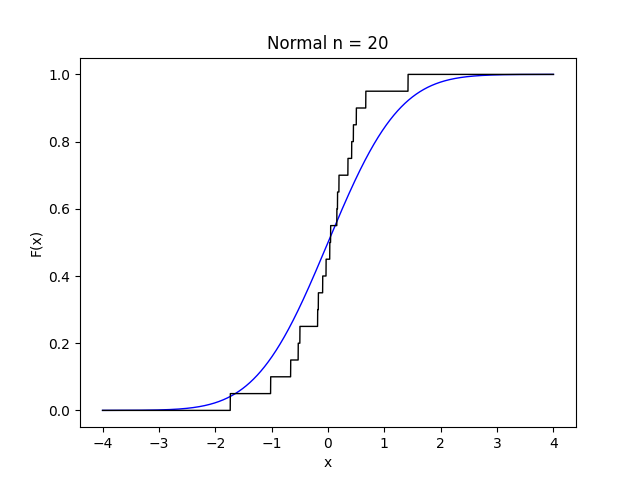
\includegraphics[scale=0.33]{normal_F20.png}
		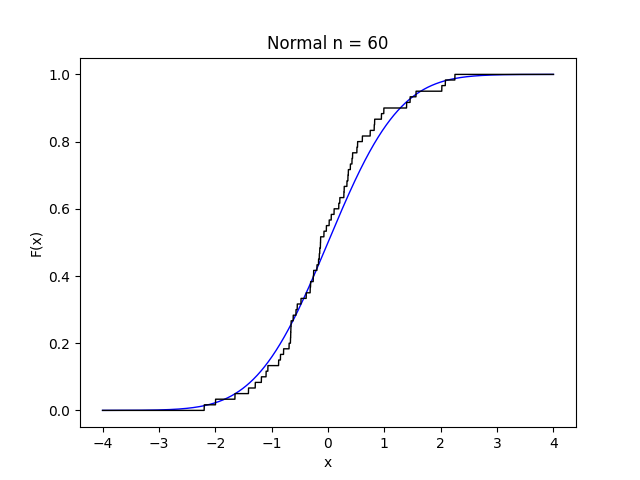
\includegraphics[scale=0.33]{normal_F60.png}
		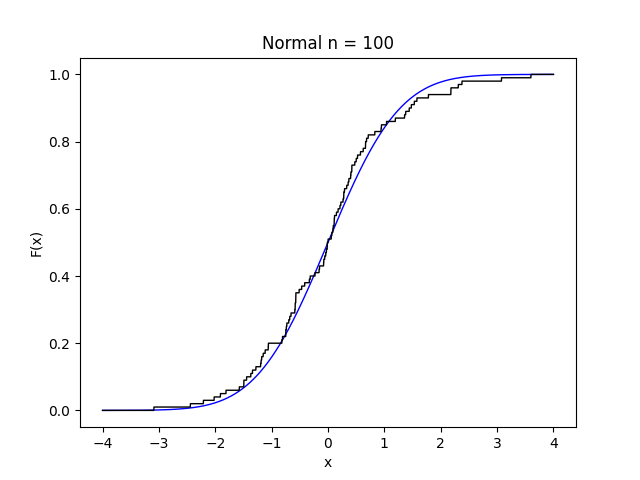
\includegraphics[scale=0.33]{normal_F100.png}
	\end{tabular}
	\caption{Функция распределения вероятности нормального р-я}
\end{figure}

\begin{figure}[H]
	\begin{tabular}{ccc}
		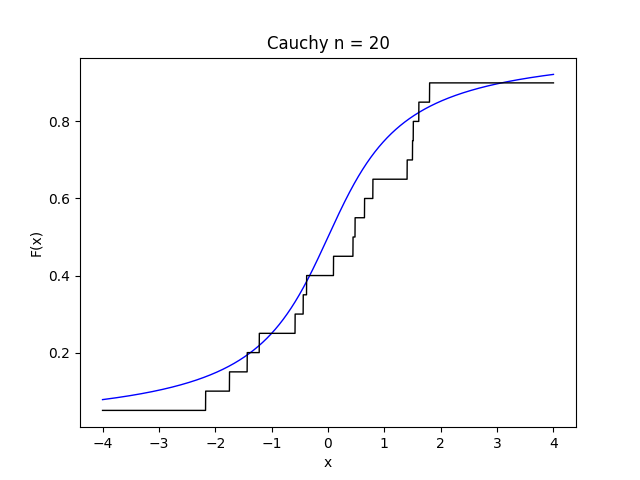
\includegraphics[scale=0.33]{cauchy_F20.png}
		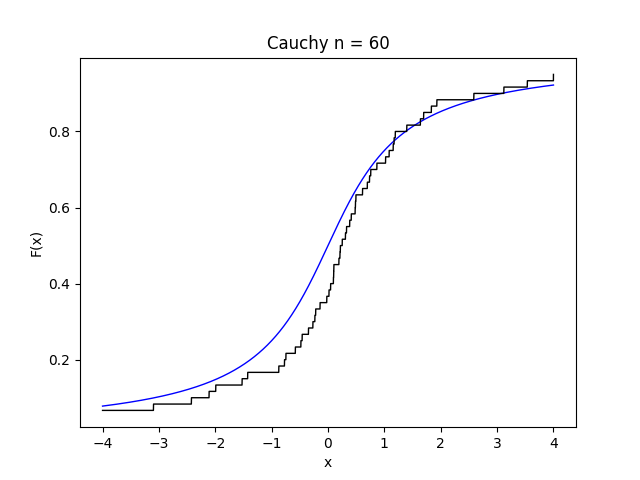
\includegraphics[scale=0.33]{cauchy_F60.png}
		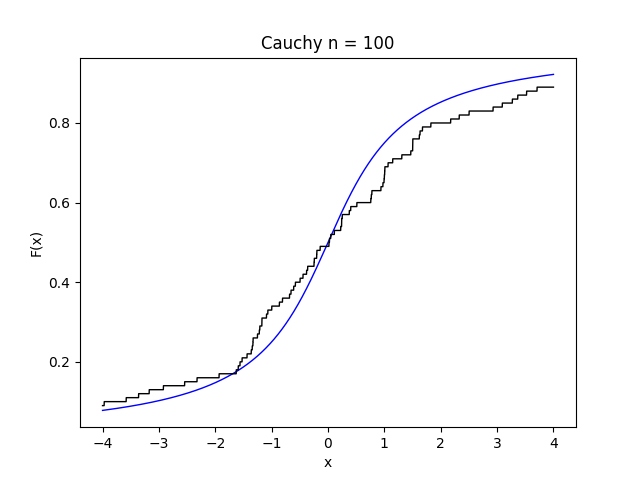
\includegraphics[scale=0.33]{cauchy_F100.png}
	\end{tabular}
	\caption{Функция распределения вероятности р-я Коши}
\end{figure}

\begin{figure}[H]
	\begin{tabular}{ccc}
		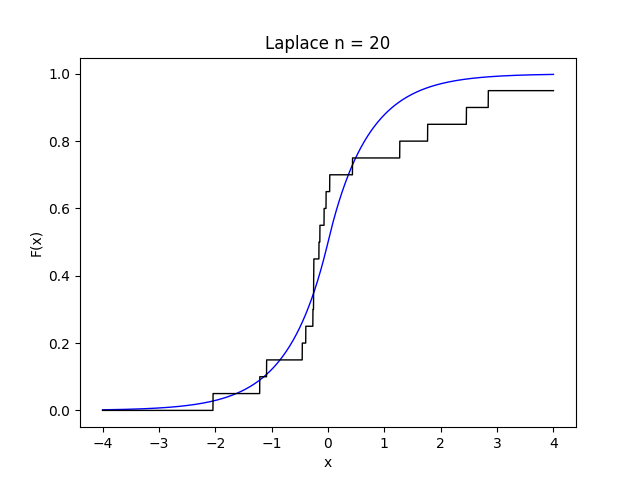
\includegraphics[scale=0.33]{laplace_F20.png}
		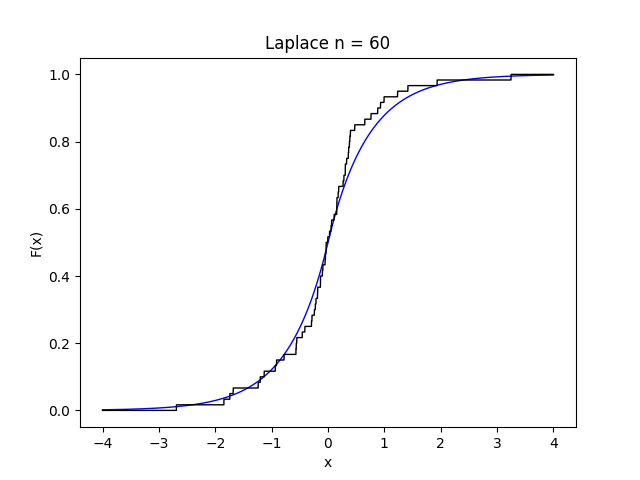
\includegraphics[scale=0.33]{laplace_F60.png}
		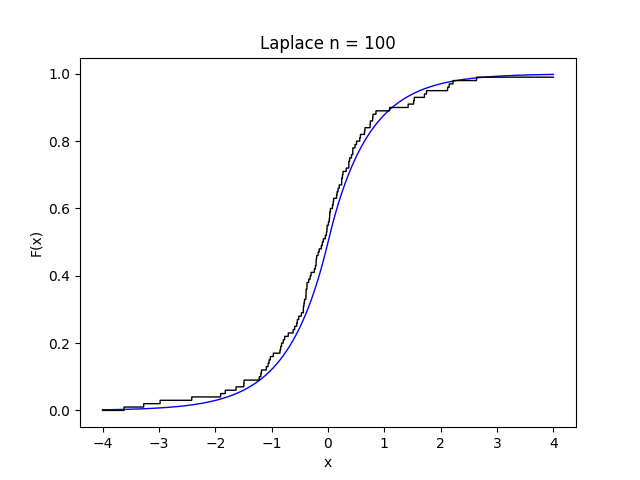
\includegraphics[scale=0.33]{laplace_F100.png}
	\end{tabular}
	\caption{Функция распределения вероятности р-я Лапласа }
\end{figure}

\begin{figure}[H]
	\begin{tabular}{ccc}
		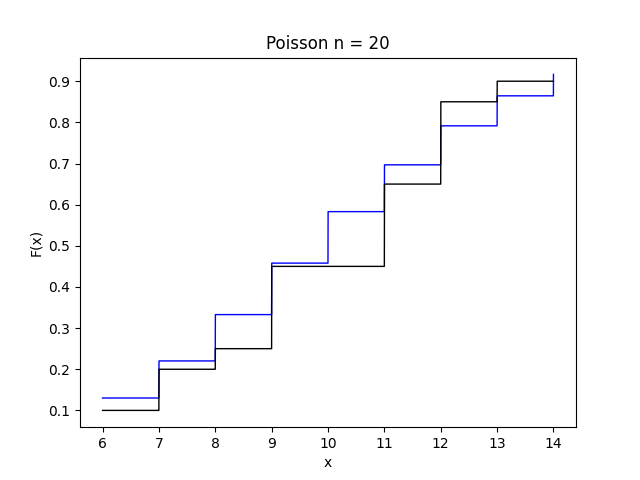
\includegraphics[scale=0.33]{poisson_F20.png}
		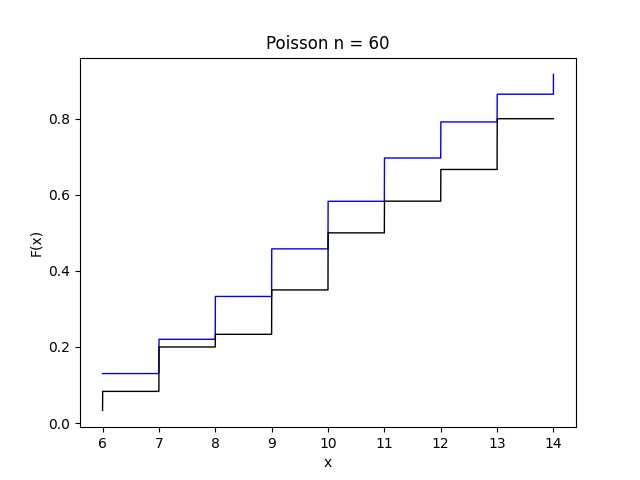
\includegraphics[scale=0.33]{poisson_F60.png}
		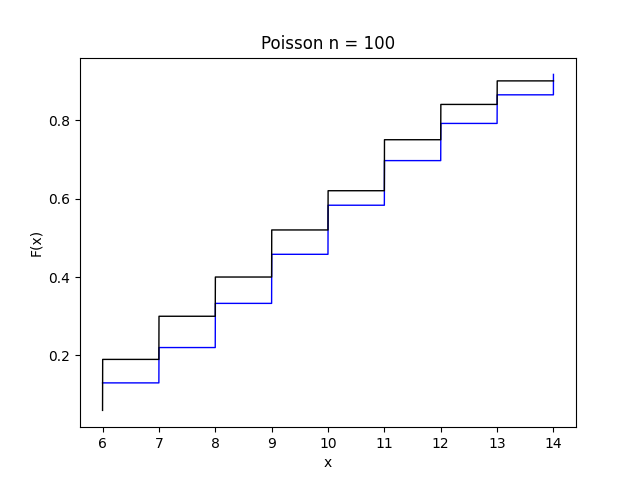
\includegraphics[scale=0.33]{poisson_F100.png}
	\end{tabular}
	\caption{Функция распределения вероятности р-я Пуассона}
\end{figure}


\begin{figure}[H]
	\begin{tabular}{ccc}
		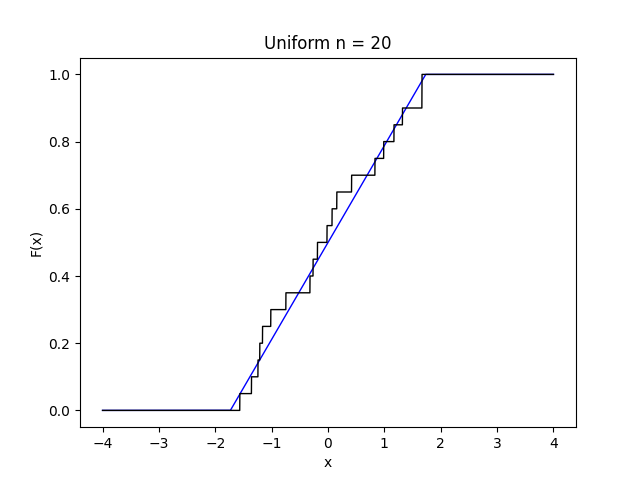
\includegraphics[scale=0.33]{uniform_F20.png}
		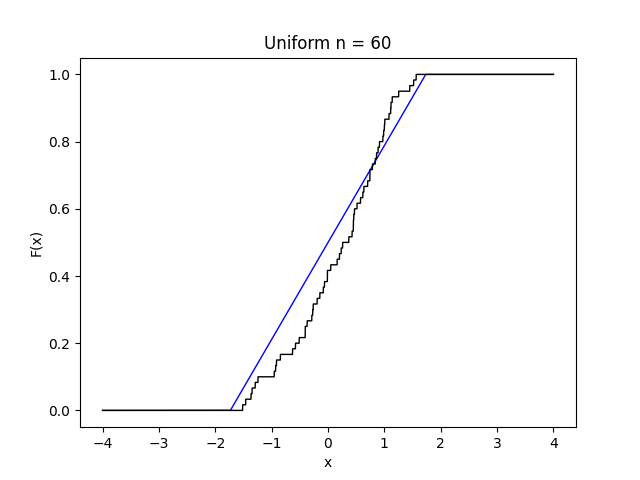
\includegraphics[scale=0.33]{uniform_F60.png}
		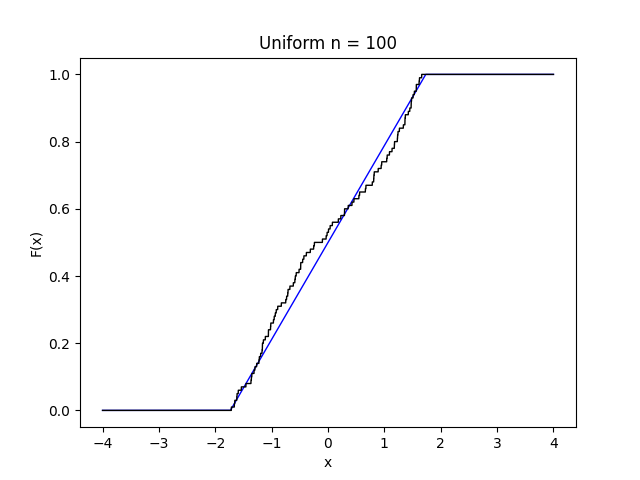
\includegraphics[scale=0.33]{uniform_F100.png}
	\end{tabular}
	\caption{Функция распределения вероятности равномерного р-я}
\end{figure}


\newpage

\section{Обсуждение}

\subsection{Гистограмма и график плотности распределения}

Исходя из результатов можно сделать вывод, что чем мощнее выборка, тем ближе ее гистограмма к графику плотности вероятности распределения, по которому данная выборка сгенерирована и тем лучше по ней можно определить характер распределения. \\
На основе выборок с маленьким размером (n=10) определить характер распределения почти невозможно. Например при n=10 невозможно отличить гистограммы равномерного распределения и распределения Пуассона. \\
Также на выборках с маленьким размером чаще наблюдаются всплески гистограмм (особенно у распределений Коши и Лапласа). 

\subsection{Характеристики положения и рассеяния}

Полученные результаты дисперсий характеристик рассеяния распределения Коши являются очень большими при всех размерах выборки. Можно сделать вывод о том, что это является следствием большого количества выбросов, которые можно также наблюдать на гистограммах. 

\subsection{Боксплот Тьюки}

Боксплоты Тьюки позволяют наглядно наблюдать характеристики распределений (например большое количество выбросов распределения Коши и отсутствия выбросов у равномерного распределения).

\subsection{Доля выбросов}

Исходя из полученых результатов мы получили что для всех распределений (за исключением нормального распределения с размером выборки 20) доли выбросов, полученные практически и теоретически приближенно равны. \\
Экспериментально и теоретически подтверждено большое количество выбросов распределения Коши, замеченное при выолнении предыдущих заданий и отсутствие выбросов у равномерного распределения.

\subsection{Эмпирическая функция распределения}

На основе полученных результатов можно сделать вывод о том, что чем больше размер выборки, тем лучше эмперическая функция распределения приближает теоретическую функцию распределения. Наибольшие отклонения при n=100 наблюдаются у распределения Пуассона.  

\subsection{Ядерные оценки плотности распределения}

На основе полученных результатов можно сделать вывод, что при увеличении размера размера выборки при всех h ядерная оценка начинает лучше приближать плотность вероятности. \\
Также можно сделать вывод, что параметр h в ядерной оценке лучше подбирать в зависимости от характера распределения. Параметр $ h = \dfrac{h_n}{2}$ лучше брать для распределений Коши и Лапласа. $h = h_n$ лучше всего походит для нормального распределения, а $ h = 2h_n $ - для распределений Пуассона и равномерного. \\
Также можно отметить, что при увеличении параметра h ядерной оценки уменьшается количество изменений знака производной. При $h=2h_n$ функция становится унимодальной. 
\newpage

\newpage
\addcontentsline{toc}{section}{Литература}

\begin{thebibliography}{4}
    \bibitem{s:hist}
    Histogram. URL: \url{https://en.wikipedia.org/wiki/Histogram}
    \bibitem{b:probSectMath}
    Вероятностные разделы математики. Учебник для бакалавров технических направлений.//Под ред. Максимова Ю.Д. --- Спб.: «Иван Федоров», 2001. --- 592 c., илл.
    \bibitem{s:boxplot}
    Box plot. URL: \url{https://en.wikipedia.org/wiki/Box_plot}
    \bibitem{a:nonParamRegr}
    Анатольев, Станислав (2009) «Непараметрическая регрессия», Квантиль, №7, стр. 37-52.
\end{thebibliography}





\end{document}